\documentclass{beamer}

\mode<presentation> {
\usetheme{Madrid}
% \usetheme{default}
% \usetheme{PaloAlto}
% \usetheme{EastLansing}
}

\beamertemplatenavigationsymbolsempty

% pacman.sty does not allow numbering pages properly with backup/appendix slides
% \usepackage{pacman}

\usepackage{graphicx} % Allows to include figures
\usepackage{booktabs} % Allows the use of \toprule, \midrule and \bottomrule in tables
% \usepackage[utf8]{inputenc}
% \usepackage{float}
% \usepackage{mathtools}
% \usepackage{xcolor}
% \usepackage{bm}
% \usepackage{scalerel}
% \usepackage{setspace}
\usepackage{tabularx}
\usepackage{appendixnumberbeamer} % add \appendix
\usepackage{tikz} % For arrow drawing

% \usepackage{amsmath}
% \usepackage{amssymb}
\usepackage{mathtools, nccmath}
% \usepackage[mathscr]{euscript}  % euler script font
% \usepackage{cleveref}
% \usepackage{enumitem}

\usepackage{algorithm}
\usepackage[noend]{algpseudocode}

\usepackage{caption}
\usepackage{subcaption}

% Custom caption style
\captionsetup{
  font=small, % Small font size for captions
  labelfont=bf, % Bold font for label (e.g., Figure 1:)
  justification=centering, % Centered caption
  singlelinecheck=false % Force centering, even for single-line captions
}

\DeclareMathOperator{\Var}{Var}
\DeclareMathOperator{\modexp}{mod\_exp}
\DeclareMathOperator{\decryptiontime}{decryption\_time}
\DeclareMathOperator{\extrareduction}{extra\ reduction}

\newcommand{\myDegree}{Master of Science Degree in Computer Science}
\newcommand{\myName}{Lorenzo Palloni}
\newcommand{\mySupervisor}{Marco Bertini}
\newcommand{\myFirstCosupervisor}{Leonardo Galteri}
\newcommand{\mySecondCosupervisor}{Donatella Merlini}
\newcommand{\myFaculty}{\protect{School of Mathematics, Physics and Natural Science}}
\newcommand{\myUni}{\protect{University of Florence}}

%---------------------------------------------------------------------------------------
%	TITLE PAGE
%---------------------------------------------------------------------------------------
\title[]{Optimization Techniques of Deep Learning Models for Visual Quality Improvement}


\author{
  \myName
}
\institute[]{
  \includegraphics[scale=0.075]{../thesis/static/logo/LOGO}\\
  % \myUni\\
  \myFaculty\\
  \myDegree\\
  \medskip
  Supervisor: \mySupervisor\\
  Co-supervisor: \myFirstCosupervisor\\
  Co-supervisor: \mySecondCosupervisor
}

\date{April 21, 2023}

\begin{document}

\begin{frame}
  \titlepage % Print the title page as the first slide
\end{frame}
%---------------------------------------------------------------------------------------

% %---------------------------------------------------------------------------------------
% % TABLE OF CONTENTS
% %---------------------------------------------------------------------------------------
% \begin{frame}
% \tableofcontents
% \end{frame}
% %---------------------------------------------------------------------------------------

%---------------------------------------------------------------------------------------
\begin{frame}{Introduction}

\begin{figure}
  \begin{columns}
    \column{0.27\textwidth}
      \includegraphics[width=0.55\linewidth]{static/crowd_original.png}
      \subcaption{{\scriptsize Original}}
    \column{0.075\textwidth}
      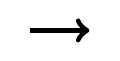
\begin{tikzpicture}
        \draw[->, line width=2.0pt] (0,0) -- (0.75,0);
      \end{tikzpicture}
    \column{0.27\textwidth}
      \includegraphics[width=0.55\linewidth]{static/crowd_compressed_blurred.png}
      \subcaption{{\scriptsize Low-resolution}}
    \column{0.075\textwidth}
      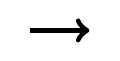
\begin{tikzpicture}
        \draw[->, line width=2.0pt] (0,0) -- (0.75,0);
      \end{tikzpicture}
    \column{0.27\textwidth}
      \includegraphics[width=0.55\linewidth]{static/crowd_srunet_int8.png}
      \subcaption{{\scriptsize Super-resolution}}
  \end{columns}
\end{figure}

\begin{itemize}
  \item Goal: Improve video restoration with deep learning models
  \item Challenge: Computational complexity of deep learning models
  \item Solution: Apply quantization techniques for faster inference and reduced memory usage
\end{itemize}
\medskip
\begin{itemize}
  \item Focus: Artefact removal and super-resolution tasks
  \item Method: Post-training quantization using TensorRT
  \item Impact: Enable practical deployment on resource-constrained devices
\end{itemize}
\end{frame}
%---------------------------------------------------------------------------------------

%---------------------------------------------------------------------------------------
\begin{frame}{Quality Metrics for Video Restoration}
\begin{itemize}
  \item Traditional Metrics:
  \begin{itemize}
%     \item PSNR, MSE, SSIM, MS-SSIM
    \item Evaluate image quality based on numerical comparisons
%     \item May not correlate well with human perception
    {\scriptsize \item An example: SSIM (Structural Similarity)}
  \end{itemize}
  \item Perceptual Metrics:
  \begin{itemize}
%     \item FID, LPIPS, LPIPS-Comp, E-LPIPS, DISTS, MOS, 2AFC, JND
    \item Evaluate image quality based on human perception
%     \item More complex to compute, but better correlation with perception
    {\scriptsize \item An example: LPIPS (Learned Perceptual Image Patch Similarity)}
  \end{itemize}
  \item No-Reference Metrics:
  \begin{itemize}
%     \item BRISQUE, NIQE, PIQUE, CONTRIQUE
    \item Evaluate image quality without reference images
    {\scriptsize \item An example: BRISQUE (Blind/Referenceless Image Spatial Quality Evaluator)}
  \end{itemize}
  \item Video Quality Metrics:
  \begin{itemize}
%     \item VMAF
    \item Take into account temporal aspects of quality degradation
    {\scriptsize \item An example: VMAF (Video Multi-Method Assessment Fusion)}
  \end{itemize}
  \end{itemize}
\end{frame}
%---------------------------------------------------------------------------------------

%---------------------------------------------------------------------------------------
\begin{frame}{Model Architectures}
\begin{itemize}
  \item UNet: encoder-decoder structure with skip connections
  \item SRUNet: modified UNet for super-resolution and artefact removal
  \item Training setup: Generative Adversarial Network (GAN) framework
  \item Generator loss: combination of LPIPS and SSIM metrics
\end{itemize}
\begin{figure}
\begin{columns}
\column{0.5\linewidth}
\includegraphics[width=0.9\textwidth]{../thesis/static/unet_architecture.png}
\subcaption{{\scriptsize UNet architecture }}
\column{0.5\linewidth}
\includegraphics[width=0.9\textwidth]{../thesis/static/srunet_architecture.png}
\subcaption{{\scriptsize SRUNet architecture }}
\end{columns}
\end{figure}
\end{frame}
%---------------------------------------------------------------------------------------

%---------------------------------------------------------------------------------------
\begin{frame}{Quantization}
  \begin{itemize}
    \item Quantization in deep learning: process of reducing the precision of weights and activations of a neural network
%     \item Goal: reduce memory footprint, computational requirements, and energy consumption
%     \item A popular choice for a quantization function is as follows:
%     \begin{itemize}
%       \item Quantized value: $Q(x) = \lfloor \frac{x - x_\mathrm{min}}{S} \rfloor$
%       \item Dequantized value: $x_{dequantized} = Q(x) \cdot S + x_\mathrm{min}$
%       \item $S$: scale factor, $x_\mathrm{min}$: minimum value
%     \end{itemize}
    \item Two main approaches to quantize a deep learning model:
    \begin{itemize}
      \item Quantization-Aware Training (QAT)
      \begin{itemize}
        \item Quantization incorporated during training
        \item Model learns to be more robust to quantization effects
      \end{itemize}
      \item Post-Training Quantization (PTQ)
      \begin{itemize}
        \item Quantization applied after training the model
        \item Model accuracy may be affected
      \end{itemize}
    \end{itemize}
  \end{itemize}
\end{frame}
%---------------------------------------------------------------------------------------

% %---------------------------------------------------------------------------------------
% \begin{frame}{Optimizations}
% \begin{itemize}
%   \item Enhancing deep learning models for super-resolution and visual artefact removal
%   \item Factors: architecture, loss functions, evaluation metrics, regularization techniques
%   \item Quantization: reduces memory footprint and computation requirements
% %   \begin{itemize}
% %     \item Uniform and non-uniform quantization
% %     \item Fixed-point, integer, and hybrid quantization
% %     \item Quantization-Aware Training (QAT) vs Post-Training Quantization (PTQ)
% %   \end{itemize}
% \end{itemize}
% \end{frame}
% %---------------------------------------------------------------------------------------

%---------------------------------------------------------------------------------------
\begin{frame}{Dataset and Training Setup}
\begin{itemize}
  \item BVI-DVC dataset:
  \begin{itemize}
    \item Designed for deep video compression tasks
    \item Includes 200 frame sequences truncated at the 64\textsuperscript{th} frame
%     \item Frame rates range from 25 to 120
    \item Various content types: natural scenes, man-made objects, cityscapes
%     \item Down-scaled versions available: 1080p, 540p, and 270p
%     \item Compressed with H.265 codec, Constant Rate Factor (CRF) of 23
  \end{itemize}
  \item Training setup:
  \begin{itemize}
    \item Models trained on frame patches of 96$\times$96 pixels randomly cropped
    \item Model training required $\sim$72 hours on a single GPU NVIDIA Titan Xp
    \item Custom data-loader: to speed up training reducing GPU bottlenecks
  \end{itemize}
\end{itemize}

\centering
\includegraphics[width=0.5\textwidth]{../thesis/static/BVI-DVC.jpg}
\captionof{figure}{{\scriptsize Some frame examples from the BVI-DVC dataset. }}

\end{frame}
%---------------------------------------------------------------------------------------

% %---------------------------------------------------------------------------------------
% \begin{frame}{Experiments}
% \begin{itemize}
%   \item Performance comparison of UNet and SRUNet models.
%   \item TensorRT optimization with different precisions: FP32, FP16, and INT8.
%   \item Quantitative results: Perceptual and traditional metrics show minor differences between optimized and non-optimized models.
%   \item Speedup: Up to 2.38X for UNet and 2.27X for SRUNet using INT8 optimization.
%   \item Memory consumption reduced up to 63.3\% for UNet and 53.8\% for SRUNet.
% \end{itemize}
% \end{frame}
% %---------------------------------------------------------------------------------------

%---------------------------------------------------------------------------------------
\begin{frame}{Experiments}
\begin{itemize}
  \item Post-Training Quantization (PTQ) implemented using TensorRT
  \item Comparison of UNet and SRUNet models with TensorRT-optimized versions (FP32, FP16, INT8)
  \item Evaluation on 60 test frames using perceptual and traditional metrics
  \item Quantitative results: Perceptual and traditional metrics show minor differences between optimized and non-optimized models.
  \item Analysis of inference speed and memory consumption
\end{itemize}
\end{frame}
%---------------------------------------------------------------------------------------

%---------------------------------------------------------------------------------------
\begin{frame}{Quantitative Results: Perceptual Metrics}
\begin{table}[htb]
  \centering
  \resizebox{\linewidth}{!}{
    \begin{tabular}{llll}
    \toprule
    {} & LPIPS $\downarrow$ & DISTS $\downarrow$ & BRISQUE $\downarrow$ \\
    \midrule
    UNet        &  \textbf{0.2897 ± 0.0138} &  \textbf{0.1222 ± 0.0067} &  31.1372 ± 1.1690 \\
    UNet-FP32   &  \textbf{0.2897 ± 0.0138} &  \textbf{0.1222 ± 0.0067} &  31.1373 ± 1.1684 \\
    UNet-FP16   &  0.2898 ± 0.0138 &  0.1223 ± 0.0067 &  31.1383 ± 1.1691 \\
    UNet-INT8   &  0.3041 ± 0.0137 &  0.1283 ± 0.0066 &  \textbf{29.6849 ± 1.0138} \\
    \midrule
    SRUNet      &  0.3111 ± 0.0151 &  \textbf{0.1717 ± 0.0047} &  27.3738 ± 3.5705 \\
    SRUNet-FP32 &  0.3111 ± 0.0151 &  \textbf{0.1717 ± 0.0047} &  27.3736 ± 3.5697 \\
    SRUNet-FP16 &  0.3111 ± 0.0151 &  \textbf{0.1717 ± 0.0047} &  27.3790 ± 3.5739 \\
    SRUNet-INT8 &  \textbf{0.3068 ± 0.0137} &  0.1722 ± 0.0044 &  \textbf{26.1546 ± 3.2273} \\
    \bottomrule
    \end{tabular}
  }
  \caption{Evaluations on perceptual metrics on 60 test frames (mean $\pm$ standard deviation).}
  \label{tab:perceptual-metrics}
\end{table}
\end{frame}
%---------------------------------------------------------------------------------------
\begin{frame}{Quantitative Results: Traditional Metrics}
\begin{table}[htb]
  \centering
  \resizebox{\linewidth}{!}{
    \begin{tabular}{llll}
    \toprule
    {} & SSIM $\uparrow$ & MS-SSIM $\uparrow$ & PSNR $\uparrow$ \\
    \midrule
    UNet        &  \textbf{0.8952 ± 0.0084} &  \textbf{0.8517 ± 0.0067} &  \textbf{21.6506 ± 0.1269} \\
    UNet-FP32   &  \textbf{0.8952 ± 0.0084} &  \textbf{0.8517 ± 0.0067} &  \textbf{21.6506 ± 0.1269} \\
    UNet-FP16   &  \textbf{0.8952 ± 0.0084} &  \textbf{0.8517 ± 0.0067} &  \textbf{21.6506 ± 0.1269} \\
    UNet-INT8   &  0.8941 ± 0.0084 &  0.8508 ± 0.0067 &  21.6388 ± 0.1286 \\
    \midrule
    SRUNet      &  \textbf{0.8894 ± 0.0084} &  \textbf{0.8457 ± 0.0062} &  21.3670 ± 0.1248 \\
    SRUNet-FP32 &  \textbf{0.8894 ± 0.0084} &  \textbf{0.8457 ± 0.0062} &  21.3670 ± 0.1248 \\
    SRUNet-FP16 &  \textbf{0.8894 ± 0.0084} &  \textbf{0.8457 ± 0.0062} &  \textbf{21.3671 ± 0.1248} \\
    SRUNet-INT8 &  0.8882 ± 0.0084 &  0.8442 ± 0.0062 &  21.3320 ± 0.1224 \\
    \bottomrule
    \end{tabular}
  }
  \caption{Evaluations on traditional metrics on 60 test frames (mean $\pm$ standard deviation).}
  \label{tab:traditional-metrics}
\end{table}
\end{frame}
%---------------------------------------------------------------------------------------
%---------------------------------------------------------------------------------------

\begin{frame}{Quantitative Results: Inference Speed}
\begin{table}[htb]
  \resizebox{0.75\linewidth}{!}{
    \begin{tabular}{llr}
    \toprule
    {}          & times [s] $\downarrow$ & speedup $\uparrow$ \\
    \midrule                                                  
    UNet        &  0.0348 ± 0.0004          &  {} \\
    UNet-FP32   &  0.0279 ± 0.0004          &  1.25X \\
    UNet-FP16   &  0.0279 ± 0.0004          &  1.25X \\
    UNet-INT8   &  \textbf{0.0146 ± 0.0006} &  \textbf{2.38X} \\
    \midrule                                                   
    SRUNet      &  0.0123 ± 0.0001          &  {} \\
    SRUNet-FP32 &  0.0087 ± 0.0005          &  1.41X \\
    SRUNet-FP16 &  0.0087 ± 0.0004          &  1.41X \\
    SRUNet-INT8 &  \textbf{0.0054 ± 0.0006} &  \textbf{2.27X} \\
    \bottomrule
    \end{tabular}
  }
  \caption{Evaluation times over 300 runs (mean $\pm$ standard deviation).}
  \label{tab:timings}
\end{table}
\end{frame}
%---------------------------------------------------------------------------------------

% %---------------------------------------------------------------------------------------
% \begin{frame}{Quantitative Results: Boxplots of Metrics}
% \includegraphics[width=1.0\textwidth]{../thesis/static/boxplots_perceptual_metrics.jpg}
% \includegraphics[width=1.0\textwidth]{../thesis/static/boxplots_traditional_metrics.jpg}
% % \includegraphics[width=\textwidth]{../thesis/static/boxplots_timings.jpg}
% % \begin{columns}
% % \column{0.5\textwidth}
% % \column{0.5\textwidth}
% % \end{columns}
% \end{frame}
% %---------------------------------------------------------------------------------------

%---------------------------------------------------------------------------------------
% \begin{frame}{Quantitative Results: Boxplots of Timings}
%   \includegraphics[width=1.0\textwidth]{../thesis/static/boxplots_timings.jpg}
% \end{frame}

%---------------------------------------------------------------------------------------
\begin{frame}{Qualitative Results: Buildings}
  % Top area
\begin{figure}
  \begin{columns}
    \column{0.33\textwidth}
      \includegraphics[width=0.6\linewidth]{static/buildings_srunet.png}
      \subcaption{Original Image (384$\times$384)}
    \column{0.33\textwidth}
      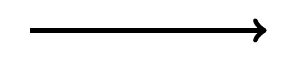
\begin{tikzpicture}
        \draw[->, line width=2.0pt] (0,0) -- (3,0);
      \end{tikzpicture}
    \column{0.33\textwidth}
      \includegraphics[width=0.15\linewidth]{static/buildings_compressed.png}
      \subcaption{Compressed and Down-scaled (96$\times$96)}
  \end{columns}

  \vspace{0.5cm} % Vertical space between top and bottom area

  % Bottom area
  \begin{columns}
    \column{0.33\textwidth}
      \includegraphics[width=0.6\linewidth]{static/buildings_bilinear_interpolation.png}
      \subcaption{Up-scaled using Bilinear Interpolation (384$\times$384)}
    \column{0.33\textwidth}
      \includegraphics[width=0.6\linewidth]{static/buildings_srunet.png}
      \subcaption{Up-scaled using SRUNet (384$\times$384)}
    \column{0.33\textwidth}
      \includegraphics[width=0.6\linewidth]{static/buildings_srunet_int8.png}
      \subcaption{Up-scaled using SRUNet-INT8 (384$\times$384)}
  \end{columns}

\end{figure}
\end{frame}
%---------------------------------------------------------------------------------------

%---------------------------------------------------------------------------------------
\begin{frame}{Qualitative Results: Crowd}
  % Top area
\begin{figure}
  \begin{columns}
    \column{0.33\textwidth}
      \includegraphics[width=0.6\linewidth]{static/crowd_srunet.png}
      \subcaption{Original Image (384$\times$384)}
    \column{0.33\textwidth}
      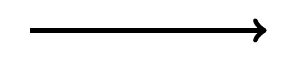
\begin{tikzpicture}
        \draw[->, line width=2.0pt] (0,0) -- (3,0);
      \end{tikzpicture}
    \column{0.33\textwidth}
      \includegraphics[width=0.15\linewidth]{static/crowd_compressed.png}
      \subcaption{Compressed and Down-scaled (96$\times$96)}
  \end{columns}

  \vspace{0.5cm} % Vertical space between top and bottom area

  % Bottom area
  \begin{columns}
    \column{0.33\textwidth}
      \includegraphics[width=0.6\linewidth]{static/crowd_bilinear_interpolation.png}
      \subcaption{Up-scaled using Bilinear Interpolation (384$\times$384)}
    \column{0.33\textwidth}
      \includegraphics[width=0.6\linewidth]{static/crowd_srunet.png}
      \subcaption{Up-scaled using SRUNet (384$\times$384)}
    \column{0.33\textwidth}
      \includegraphics[width=0.6\linewidth]{static/crowd_srunet_int8.png}
      \subcaption{Up-scaled using SRUNet-INT8 (384$\times$384)}
  \end{columns}

\end{figure}
\end{frame}
%---------------------------------------------------------------------------------------

%---------------------------------------------------------------------------------------
% \begin{frame}{Qualitative Results}
% \includegraphics[width=\textwidth]{../thesis/static/03_srunet_qualitative_results.png}
% \end{frame}
%---------------------------------------------------------------------------------------

% \begin{frame}{Inference Speed and Qualitative Results}
% \begin{columns}
% \column{0.5\textwidth}
% % \caption{Inference Speed}
% % \column{0.5\textwidth}
% % \caption{Qualitative Results: Trees (UNet)}
% \includegraphics[width=\textwidth]{../thesis/static/03_srunet_qualitative_results.png}
% \end{columns}
% \end{frame}
% %---------------------------------------------------------------------------------------

%---------------------------------------------------------------------------------------
\begin{frame}{Conclusions}
\begin{itemize}
  \item Aim to optimize deep learning models for video quality improvement
  \item Investigated post-training quantization techniques using TensorRT
  \medskip
  \item Achieved up to 2.38X speedup and 64.3\% size reduction without compromising performance
  \medskip
  \item Future research:
    \begin{itemize}
      \item designing efficient NN model architectures
      \item co-designing NN architecture and hardware together
      \item pruning
      \item knowledge distillation
      \item exploring different quantization techniques
    \end{itemize}
\end{itemize}
\end{frame}
%---------------------------------------------------------------------------------------

%---------------------------------------------------------------------------------------
% DO-YOU-HAVE-ANY-QUESTIONS
%---------------------------------------------------------------------------------------
\begin{frame}  % [c,noframenumbering]

{\Huge \emph{Thank you, for your attention!}}

\begin{itemize}
  \item[]
  \item[]
\end{itemize}

\LARGE Do you have any questions?

\begin{itemize}
  \item[]
\end{itemize}

\begin{columns}
\column{0.5\textwidth}
\column{0.5\textwidth}
\includegraphics[width=\linewidth]{../thesis/static/logo/LOGO}\\
\end{columns}

\end{frame}
%---------------------------------------------------------------------------------------

% %---------------------------------------------------------------------------------------
% % BIBLIOGRAPHY
% %---------------------------------------------------------------------------------------
% \begingroup
% \footnotesize
% \begin{frame}[noframenumbering]{References}
% \begin{thebibliography}{99}
% 
% % \bibitem{bib:kocher}{Kocher, P.C., 1996, August. Timing attacks on implementations of Diffie-Hellman, RSA, DSS, and other systems. In Annual International Cryptology Conference (pp. 104-113). Springer, Berlin, Heidelberg.}
% % \bibitem{bib:openssl}{Brumley, D. and Boneh, D., 2005. Remote timing attacks are practical. Computer Networks, 48(5), pp.701-716.}
% % \bibitem{bib:boreale}{Boreale, M., 2003. Note per il corso di Sicurezza delle Reti.}
% % \bibitem{bib:montgomery}{Montgomery, P.L., 1985. Modular multiplication without trial division. Mathematics of computation, 44(170), pp.519-521.}
% % \bibitem{bib:sliding}{Menezes, A.J., Van Oorschot, P.C. and Vanstone, S.A., 2018. Handbook of applied cryptography. CRC press.}
% % \bibitem{bib:schindler}{Schindler, W., 2000, August. A timing attack against RSA with the chinese remainder theorem. In International Workshop on Cryptographic Hardware and Embedded Systems (pp. 109-124). Springer, Berlin, Heidelberg.}
% % \bibitem{bib:coppersmith}{Coppersmith, D., 1997. Small solutions to polynomial equations, and low exponent RSA vulnerabilities. Journal of cryptology, 10(4), pp.233-260.}
% 
% \end{thebibliography}
% \end{frame}
% \endgroup
% %---------------------------------------------------------------------------------------

%---------------------------------------------------------------------------------------
% APPENDIX
%---------------------------------------------------------------------------------------
\appendix
\begin{frame}[c,noframenumbering]

  \Huge Appendix

\end{frame}

%---------------------------------------------------------------------------------------
\begin{frame}{Quantitative Results: VMAF}
\begin{table}[htb]
  \centering
  \resizebox{\linewidth}{!}{
    \begin{tabular}{llll}
    \toprule
    {} &       VMAF (mean) $\uparrow$ &  VMAF (harmonic mean) $\uparrow$ \\
    \midrule
    UNet        &  47.71 &      47.20 \\
    UNet-FP32   &  \textbf{47.72} &      \textbf{47.21} \\
    UNet-FP16   &  47.71 &      47.20 \\
    UNet-INT8   &  47.47 &      46.96 \\
    \midrule
    SRUNet      &  \textbf{47.20} &      \textbf{46.65} \\
    SRUNet-FP32 &  47.19 &      46.64 \\
    SRUNet-FP16 &  47.19 &      \textbf{46.65} \\
    SRUNet-INT8 &  47.18 &      46.64 \\
    \bottomrule
    \end{tabular}
  }
  \caption{VMAF scores on a 120-second-test video.}
  \label{tab:vmaf}
\end{table}
\end{frame}
%---------------------------------------------------------------------------------------

%---------------------------------------------------------------------------------------
\begin{frame}{Qualitative Results: Trees}
  % Top area
\begin{figure}
  \begin{columns}
    \column{0.33\textwidth}
      \includegraphics[width=0.6\linewidth]{static/trees_srunet.png}
      \subcaption{Original Image (384$\times$384)}
    \column{0.33\textwidth}
      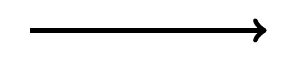
\begin{tikzpicture}
        \draw[->, line width=2.0pt] (0,0) -- (3,0);
      \end{tikzpicture}
    \column{0.33\textwidth}
      \includegraphics[width=0.15\linewidth]{static/trees_compressed.png}
      \subcaption{Compressed and Down-scaled (96$\times$96)}
  \end{columns}

  \vspace{0.5cm} % Vertical space between top and bottom area

  % Bottom area
  \begin{columns}
    \column{0.33\textwidth}
      \includegraphics[width=0.6\linewidth]{static/trees_bilinear_interpolation.png}
      \subcaption{Up-scaled using Bilinear Interpolation (384$\times$384)}
    \column{0.33\textwidth}
      \includegraphics[width=0.6\linewidth]{static/trees_srunet.png}
      \subcaption{Up-scaled using SRUNet (384$\times$384)}
    \column{0.33\textwidth}
      \includegraphics[width=0.6\linewidth]{static/trees_srunet_int8.png}
      \subcaption{Up-scaled using SRUNet-INT8 (384$\times$384)}
  \end{columns}

\end{figure}
\end{frame}
%---------------------------------------------------------------------------------------

%---------------------------------------------------------------------------------------
\begin{frame}{LPIPS-Comp: Introduction (1/5)}
  \begin{itemize}
    \item LPIPS-Comp: perceptual similarity metric based on deep neural networks
    \item Trained on a compression-specific perceptual similarity dataset
    \item Better alignment with human judgement on general compression tasks
  \end{itemize}
\end{frame}

\begin{frame}{VGG-16 and Feed-Forward Process (2/5)}
  \begin{itemize}
    \item LPIPS-Comp uses VGG-16 architecture
    \item ReLU activations after each conv block in the first five layers
    \item Batch-normalization applied
    \item Feed-forward performed on VGG-16 for both original ($y$) and reconstructed image ($\hat{y}$)
  \end{itemize}
\end{frame}

\begin{frame}{Feature Activations and Normalization (3/5)}
  \begin{itemize}
    \item $F(y)$ and $F(\hat{y})$ return stacks of feature activations for all layers $L$
    \item Unit-normalized in the channel dimension: $z^l_y, z^l_{\hat{y}} \in R^{H_l \times W_l \times C_l}$ where $l \in L$
    \item $H_l, W_l$ are the spatial dimensions; $C_l$ is the number of channels
  \end{itemize}
\end{frame}

\begin{frame}{Scaling and L2 Distance (4/5)}
  \begin{itemize}
    \item $z^l_y , z^l_{\hat{y}}$ are scaled channel-wise with the vector $w_l \in R^{C_l}$
    \item L2 distance computed and averaged over spatial dimensions
    \item Channel-wise sum performed
  \end{itemize}
\end{frame}

\begin{frame}{LPIPS-Comp Equation (5/5)}
  $$ \text{LPIPS-Comp}(y, \hat{y}) = \sum_{l} \frac{1}{H_l W_l} \sum_{h, w} \left| \left| w_l \odot \left( z^l_{\hat{y}, h, w} - z^l_{y, h, w} \right) \right| \right|^2_2 $$
  \begin{itemize}
    \item Weights in $F$ learned for image classification and kept fixed
    \item $w$ are linear weights learned on a compression-specific similarity dataset
  \end{itemize}
\end{frame}
%---------------------------------------------------------------------------------------

\end{document}

